\documentclass{article}

\usepackage{amsthm}
\usepackage{amsmath}
\usepackage{graphicx}
\usepackage{verbatim}
\usepackage{amssymb}
\usepackage{float}

\def\refname{Referinte}

\graphicspath{{res/}}

\newtheorem{fig}{Figura}[section]
\newtheorem{definition}{Definitie}[section]
\newtheorem{prop}{Propozitie}[section]
\newtheorem{example}{Exemplu}[section]
\newtheorem{explanado}{Explicatie}[section]

\renewcommand{\figurename}{Figura}

\begin{document}

\title{Logica si Deep Learning}
\author{Chris Luntraru}
\date{}
\maketitle

\begin{abstract}
Acest referat ilustreaza modelul ``Logic Tensor Network'' propus de Luciano Serafini si Artur d'Avila Garcez cu scopul de a automatiza rationalizarea si invatarea pe retele neurale. Este definit un formalism logic numit ``Real Logic'' (Logica reala), bazat pe un limbaj al logicii de ordinul intai, unde formulele au valori de adevar reprezentate de numere reale cuprinse in intervalul [0, 1]. Logica reala implementata in Retele Neurale Tensoriale permite rationarea deductiva, plecand de la o baza de cunostinte. Prezentarea acestor notiuni incepe cu o scurta ilustrare a retelelor neurale si a tensorilor, precum si a retelelor neurale tensoriale. Mai departe, este realizata o scurta introducere in logica de ordinul I pe care se bazeaza logica reala, ce ajuta la definirea retealei logice tensoriale.
\end{abstract}

\section{Introducere}
Exista o multitudine de baze de cunostinte precum WordNet si Google Knowledge Graph, utilizate pentru cautarea unor date, oferirea unor informatii structurate utilizatorului sau pentru a oferi raspunsuri la intrebari. Aparitia acestor servicii a determinat accentuarea cercetarii pe dezvoltarea unor baze de cunostinte plecand de la un set de informatii cunoscute. Ideea pe care se bazeaza modelul este acela de a implementa o forma de ``bun simt'', o simulare a gandirii umane pentru a deduce anumite concluzii din informatii incomplete. Omul dispune de aceasta capacitate care ii este extrem de utila la ordinul zilei. Pentru a exemplifica, putem considera un caz in care o persoana oarecare primeste informatia ca o noua specie de maimuta a fost descoperita. Nu este necesar ca acestuia sa ii fie confirmat ca si aceasta noua maimuta va avea picioare, maini, etc. \cite{NTN} Recent, in domeniul machine learningului, se poate observa un accent pus pe completarea bazelor de cunostinte, deductii aproximate si rationalizare bazata pe statistici si retele neurale. \cite{LTN}

\section{Reteaua neurala artificiala}
Retelele neurale artificiale sunt, conform numelui, modelate dupa sistemul nervos al omului. Acestea fiind spuse, cea mai intuitiva componenta a unei astfel de retele este neuronul artificial. \cite{Deep_Learning}

\begin{figure}[H]
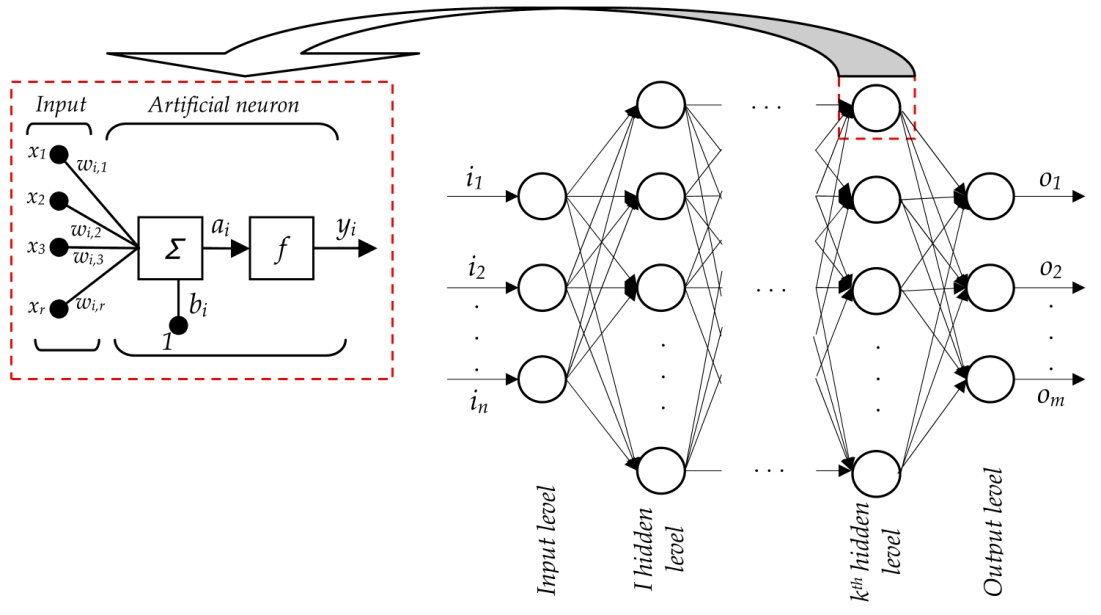
\includegraphics{ANN_Structure}
\caption{Retea neurala si neuron artificial \cite{Deep_Learning}}
\end{figure}

O retea neurala e impartita intr-un numar de straturi (Layers). Primul se numeste ``Input Layer'', ultimul ``Output Layer'', iar restul ``Hidden Layer''. Aceste denumiri reflecta scopul fiecareia dintre ele: primul strat se comporta altfel decat celelalte, nu au o functie care proceseaza informatiile primite, ci pur si simplu furnizeaza informatii constante pentru urmatorul strat. Stratul de output intoarce informatiile relevante pentru utilizator. Cele ascunse sunt denumite astfel datorita faptului ca o persoana nu poate urmari cum sunt procesate datele in acestea, ca urmare a numarului ridicat al neuronilor prezenti.

\subsection{Functionarea unui neuron}

\begin{figure}[H]
	\includegraphics[scale=0.5]{neuron_s}
	\caption{Neuron Artificial \cite{Deep_Learning}}
\end{figure}

In Figura 1 se poate observa structura unui neuron artificial:\\

\begin{itemize}
	\item $x_1, x_2, ..., x_n$ sunt inputuri. \\
	\item $w_0, w_1, w_2, ..., w_n$ sunt ``greutati'' ale fiecareia dintre muchii. \\
	\item $x0$ este coeficientul  ``bias'', si are de obicei valoarea $+1$, $w_0$ fiind cel responsabil pentru efectul lui asupra rezultatului.\\
	\item $a$ este outputul functiei de activare.\\
\end{itemize}

Outputul unui neuron artificial este calculat astfel:\\
$a = \sigma(\sum_{i=0}^n w_i x_i)$

\begin{example}
Putem exemplifica functionarea unei retele neurale prin calcularea unei operatii simple precum AND logic. Structura neuronului pentru functie se poate observa in figura 3. In acest caz, intreaga retea este un singur neuron datorita naturii simple a operatiei. Functia de activare, in acest caz va fi:\\
\[
	\sigma(x)= \left\{
	\begin{array}{ll}
	$0, daca  x $<$ 0$\\
	$1, daca x $\geq$ 0$
	\end{array}
	\right.
\]\\
inputurile $x_1, x_2$ vor fi cele date de utilizator, iar $b = -1.5$.\\
Asadar, outputul $a = \sigma(-1.5+x1+x2)$

\begin{figure}[H]
	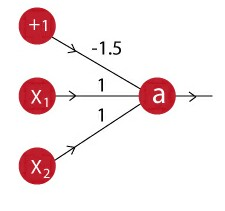
\includegraphics[scale=0.5]{and_s}
	\caption{Retea pentru AND \cite{Deep_Learning}}
\end{figure}

\begin{figure}[H]
	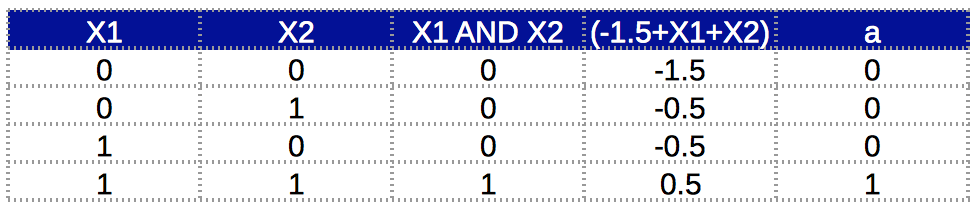
\includegraphics[scale=0.5]{and_table}
	\caption{Tabel de adevar pentru AND si $\sigma$ \cite{Deep_Learning}}
\end{figure}

\end{example}

\begin{example}
Un exemplu mai complex, la care este nevoie sa folosim mai multi neuroni pentru a alcatui reteaua este cea pentru $\neg (x_1 \oplus x_2)$:\\
$\neg (x_1 \oplus x_2) = \neg((x_1+x_2) \land (\neg x_1 + \neg x_2))$

\begin{figure}[H]
	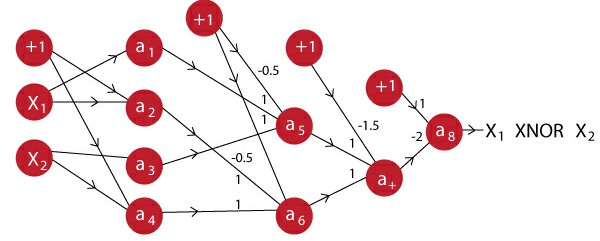
\includegraphics[scale=0.5]{xnor_s}
	\caption{Reteaua neurala pt XNOR \cite{Deep_Learning}}
\end{figure}

\end{example}

\subsection{Backpropagation}
Algoritmul pe care se bazeaza retelele neurale pentru a minimiza eroarea calculelor se numeste ``Backpropagation'' \cite{Deep_Learning}. Numele este sugestiv, intrucat se updateaza greutatile muchiilor plecand de la eroarea rezultatului furnizat de retea. Pentru a intelege cum functioneaza algoritmul, trebuie sa definim derivata partiala.

\begin{figure}[H]
	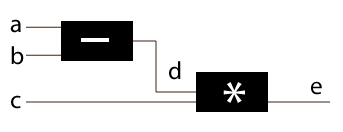
\includegraphics[scale=0.5]{gradient_diagram}
	\caption{Derivata partiala in reteaua neurala \cite{Deep_Learning}}
\end{figure}

\begin{definition}[Derivata Partiala]
Derivata partiala a unei functii in raport cu o variabila este viteza cu care se modifica in functie de acea variabila. \cite{Deep_Learning}\\
\end{definition}

\begin{example}
In Figura 6, se poate observa o retea neurala simpla, pentru care vom calcula derivatele partiale ale functiei $f(a, b, c) = (a - b) \cdot c$. Notam $d = a + b$ si $e = d \cdot c$:\\
$\cfrac{\partial e}{\partial d} = c$\ \ \ \ 
$\cfrac{\partial e}{\partial c} = d$\\ \\
$\cfrac{\partial d}{\partial a} = 1$\ \ \ \ 
$\cfrac{\partial d}{\partial b} = -1$\\ \\
Pentru a calcula derivatele partiale in functie de a si b, insa, trebuie sa utilizam operatii algebrice simple:\\
$\cfrac{\partial e}{\partial a} = \cfrac{\partial e}{\partial d} \cdot \cfrac{\partial d}{\partial a} = c$ \\ \\ 
$\cfrac{\partial e}{\partial b} = \cfrac{\partial e}{\partial d} \cdot \cfrac{\partial d}{\partial b} = -c$ \\
\end{example}

Astfel, stim efectul fiecarui nod asupra rezultatului final dat de retea si putem incepe sa ``antrenam'' reteaua.

\begin{definition}[Antrenament]
``Antrenamentul'' unei retele neurale se refera la rularea	 retelei pe un set de date pentru care este cunoscut rezultatul si modificarea greutatilor muchiilor cu valori mici, pentru a apropia rezultatul de cel asteptat. 
\end{definition}

Greutatea unei variabile $x$ va fi modificata in functie de derivata partiala a retelei in raport cu $x$ si in functie de eroarea neuronului.\\
Eroarea neuronului va fi calculata in functie de eroarea stratului urmator.

\section{Tensorul}

\begin{definition}[Tensor]
Un tensor de rang r si ordin n este un obiect matematic cu n indici si $n^r$ componente. \cite{Tensor}
\end{definition}

\begin{prop}
Ordinul n al unui tensor reprezinta numarul de dimensiuni al spatiului in care se afla. \cite{Tensor}
\end{prop}

\begin{prop}
Rangul r al unui tensor reprezinta numarul de directii determinate de acesta. \cite{Tensor_Rank}
\end{prop}

\begin{prop}
	Fie v1 si v2 tensori de rang 1 si ordin 3, astfel incat sa fie reprezentati de vectorii tridimensionali:\\
	$v_1 = a_1 \cdot \vec{i} + b_1 \cdot \vec{j} + c_1 \cdot \vec{k}$\\
	$v_2 = a_2 \cdot \vec{i} + b_2 \cdot \vec{j} + c_2 \cdot \vec{k}$\\
	Produsul acestor tensori \cite{Tensor_Multiplication} se calculeaza similar cu produsul polinoamelor care le reprezinta, cu mentiunea ca se obtine un tensor de rang 2 si ordin 3:\\
\begin{align*}
	\overrightarrow{\overrightarrow{v_1 v_2}} = &a_1 a_2 \overrightarrow{\overrightarrow{ii}} + a_1 b_2 \overrightarrow{\overrightarrow{ij}} + a_1 c_2 \overrightarrow{\overrightarrow{ik}}\\
	&b_1 a_2 \overrightarrow{\overrightarrow{ji}} + b_1 b_2 \overrightarrow{\overrightarrow{jj}} + b_1 c_2 \overrightarrow{\overrightarrow{jk}}\\
	&c_1 a_2 \overrightarrow{\overrightarrow{ki}} + c_1 b_2 \overrightarrow{\overrightarrow{kj}} + c_1 c_2 \overrightarrow{\overrightarrow{kk}}\\
\end{align*}
, unde $\overrightarrow{\overrightarrow{ii}}, \overrightarrow{\overrightarrow{ij}},...,\overrightarrow{\overrightarrow{kk}}$ sunt tensorii unitate de ordin 2. Tensorul rezultat se poate reprezenta cu ajutorul matricei:\\
 \[
   M=
  \left[ {\begin{array}{ccc}
  	a_1 a_2	 & a_1 b_2 & a_1 c_2 \\
	b_1 a_2	 & b_1 b_2 & b_1 c_2 \\
	c_1 a_2	 & c_1 b_2 & c_1 c_2 \ 
  \end{array} } \right]
\]
\end{prop}

\begin{prop}
Inmultirea tensorilor se generalizeaza, un tensor de rang r si ordin n obtinandu-se prin inmultirea a r tensori de ordin n.
\end{prop}

\section{Reteaua neurala tensoriala}
Modelul este introdus in articolul \cite{NTN}. Acesta incearca sa implementeze o forma de ``bun simt'' in retele neurale, interpretat sub forma prezicerii unor relatii bazat pe un set de cunostinte. In alte cuvinte, are scopul de a putea determina daca doua entitati e1 si e2 se afla intr-o relatie R, plecand de la o baza de date. Pentru a obtine acest scop, reprezentam entitatile ca tensori cu rolul de a descrie respectivele obiecte. Aduce in plus fata de modelul retelelor neurale ``clasice'' un mod direct de a stabili o relatie dintre obiecte, fata de a concatena pur si simplu vectorii-entitate inainte de a lucra cu ei.

\begin{definition}[Retea Neurala Tensoriala]
O retea neurala tensoriala este o retea neurala ce considera obiectele din input tensori n-dimensionali de rang 1. 
\end{definition}

\begin{prop}
Din moment ce tensorii considerati in situatia de fata au rangul 1, pot fi vizualizati ca vectori de forma $v \in \mathbf{R}^n$. Astfel, putem reprezenta comod atributele numerice ale unui obiect ca marimi pe o anumita dimensiune.
\end{prop}

\begin{example}
Fie O multimea persoanelor caracterizate prin inaltime, greutate si sex. Consideram inaltimea in cm, greutatea in kg, si sexul ca o valoarea booleana (0 pentru masculin si 1 pentru feminin). Astfel, un barbat de 1.8m care cantareste 75kg va fi reprezentat ca:\\
$v = <180, 75, 0> \in \mathbf{R}^3$
\end{example}

Functia care determina probabilitatea ca 2 entitati sa fie in relatie una cu cealalta are forma urmatoare \cite{NTN}: \\ \\
$g(o_1, R, o_2) = U_R^T tanh(o_1^T W_R^{[1:k]}o_2 + V_R \left[\begin{smallmatrix} o_1 \\ o_2 \end{smallmatrix}\right] + b_R)$, unde:\\
\begin{itemize}
	\item tanh = tangenta hiperbolica, o functie nonliniara standard
	\item k este numarul de ``interpretari'' ale relatiei R (ex: O masina poate avea o componenta (roata), dar si un caine poate (picior))
	\item $W_R^{[1:k]}$ este un tensor
	\item produsul $o_1^T W_R^{[1:k]}o_2$ rezulta intr-un vector k-dimensional de scalari care, trecuti prin functia tanh si celelalte operatii, vor fi in intervalul [0, 1]
\end{itemize}

Ceilalti parametri apartin formei standard a retelei neurale \cite{NTN}:\\
\begin{itemize}
	\item e1 si e2 cele 2 obiecte pentru care stabilim daca se afla in relatia R
	\item d numarul de dimensiuni al entitatilor e1 si e2
	\item $V_R \in \mathbf{R}^{k \cdot 2d}$, unde $V_R \left[\begin{smallmatrix} o_1 \\ o_2 \end{smallmatrix}\right]$ stabileste relatia dintre e1 si e2 concatenand vectorii (metoda clasica)
	\item $U_R \in \mathbf{R}^k$ se inmulteste cu vectorul k-dimensional pentru a obtine un scalar, numar real in [0, 1]
	\item $b_R \in \mathbf{R}^k$ ``bias''ul
\end{itemize}

\begin{figure}[H]
	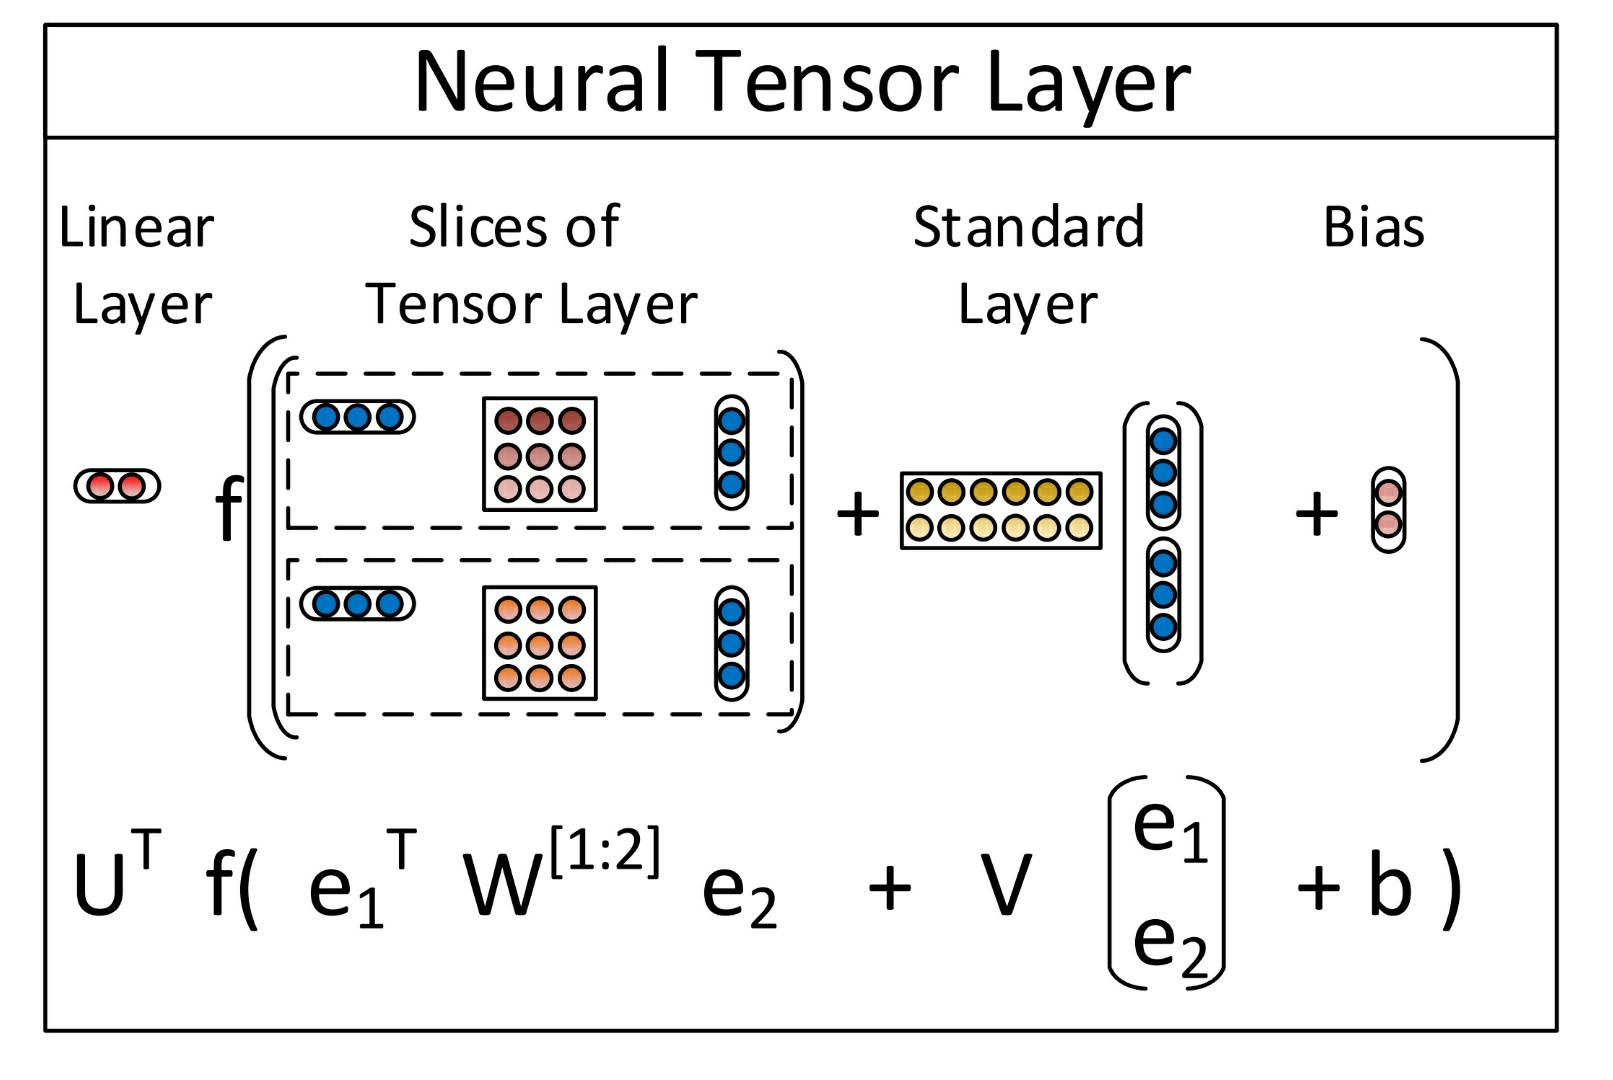
\includegraphics[scale=0.15]{ntn_rep}
	\caption{Reprezentare grafica a formulei \cite{NTN}}
\end{figure}

\section{O prezentare scurta a logicii de ordinul I}
Cateva notiuni elementare ce apartin logicii de ordinul sunt necesare pentru a intelege reteaua tensoriala logica. Desi cursul prezinta logica propozitionala, consider ca acesta acopera totusi cea mai mare parte din materia necesara pentru a putea trece mai departe. Asadar, aceasta prezentare foarte scurta, cuprinzand doar cateva simboluri si un exemplu pentru a acomoda cititorul cu conceptul.

\begin{definition}[Limbajul de ordinul I]
Simbolurile unui limbaj de ordinul intai $\mathcal{L}$ sunt \cite{FOL}:\\
\begin{itemize} 
	\item o multime de simboluri pentru functii, de aritati specificate
	\item o multime de simboluri pentru relatii precum =
	\item o multime de simboluri pentru constante
	\item quantificatorii ``oricare ar fi'' ($\forall$) si ``exista'' ($\exists$)
	\item o multime infinita de variabile $v_0, v_1, ..., v_n, \forall n \in \mathbf(N)$
	\item conectorii propozitionali precum $\neg, \land, \lor$
	\item paranteze si virgula (,)
\end{itemize}
\end{definition}

\begin{definition}[Termen]
Un termen t al unui limbaj $\mathcal{L}$ este o variabila sau constanta a unui limbaj. \cite{FOL}
\end{definition}

\begin{definition}[Clauza]
O clauza $\phi$ a unui limbaj $\mathcal{L}$ este o expresie formata dintr-un numar de formule atomice (sau negatiile lor) adevarata daca oricare dintre componente este adevarata. \cite{Clause}
\end{definition}

\begin{prop}
O clauza $\phi$ de obicei reprezentata sub forma:\\
	$\phi = \phi_1 \vee \phi_2 \vee ... \phi_k$, unde $k \in \mathbf{N}$ este numarul de atomi sau negatii de atomi. \cite{Clause}
\end{prop}

\begin{definition}[Termen inchis/Clauza inchisa]
Un termen inchis/ o clauza inchisa este un termen/ o clauza ce nu contine variabile. \cite{Closed_Term}
\end{definition}

\begin{definition}[Variabila libera]
O variabila dintr-o formula este libera daca nu are cuantificator. \cite{Free_Variable}
\end{definition}

\begin{example}
In formula $\forall yP(x, y)$, x este variabila libera.\cite{Free_Variable}
\end{example}

\begin{example}
Fie variabilele x si y si functiile:\\
friend(x, y) = x si y sunt prieteni\\
smoke(x) = x fumeaza\\
cancer(x) = x are cancer\\ \\
Atunci, expresia:\\
$\forall xy(friend(x,y) \land smoke(x)) \rightarrow smoke(y)$ \\
se citeste ``Pentru orice x si y cu x si y sunt prieteni si x fumeaza, y fumeaza.''
\end{example}

\section{Reteaua tensoriala logica}
Scopul acestui model este acela de a introduce un mod adecvat de a implementa invatarea si rationalizarea intr-un mod usor de integrat intr-un agent (de exemplu, o masina care se conduce singura). Acest agent trebuie sa lucreze cu informatii dintr-o multime, potential infinita, de obiecte $\mathcal{O} = {o_1, o_2, ...}$. Obiectele sunt asociate cu un set de atribute reprezentate numeric, prin intermediul unor vectori n-dimensionali (tensori de rang 1 si ordin n). Aceste tupluri pot participa intr-o multime de relatii $\mathcal{R} = {R_1, R_2, ..., R_k}$, unde $R_i \subseteq \mathcal{O}^{\alpha(R_i)}$, unde $\alpha(R_i)$ este aritatea relatiei $R_i$. Se considera cunoscute \cite{LTN}:\\
\begin{itemize}
	\item ca exista o relatie intre aceste proprietati numerice 
	\item o retea de relatii $\mathcal{R}$ in $\mathcal{O}$. 
\end{itemize}

Plecand de la aceste cunostinte incomplete, agentul are rolul de a deduce \cite{LTN}:\\
\begin{itemize}
	\item noi informatii despre reteaua de relatii intre obiectele din $\mathcal{O}$
	\item proprietatile numerice sau clasele obiectelor din $\mathcal{O}$
\end{itemize}
unde clasa unui obiect se refera la categoria din care face parte. De exemplu daca definim pe limbajul $\mathcal{L}$ clasele adult, copil, persoana, expresia ($persoana(x) \wedge (adult(x) \vee copil(x))$) va fi adevarata. De cele mai multe ori, clasele si relatiile nu sunt independente. Mai exact, daca un obiect x este de clasa C (C(x)), si se afla in relatia R cu y, atunci putem deduce, in anumite contexte C(y). Valoarea de adevar a C(y) depinde de situatie. Astfel se poate intampla sa deducem C(y) din exemple de ``antrenament'', dar odata ce acumulam mai multe cunostinte sa fie nevoie sa revizuim aceasta concluzie. Aceste idei sunt implementate cu ajutorul retelelor tensoriale in timp ce se folosesc de puterea logicii de ordinul I de a reprezenta afirmatii.


Reteaua tensoriala logica introdusa in articolul \cite{LTN} se bazeaza pe o noua paradigma a logicii, numita ``Real logic'' (Logica reala).

\subsection{Logica Reala}
Plecam de la un limbaj de ordinul I $\mathcal{L}$ ce contine \cite{LTN}:\\
\begin{itemize}
	\item $\mathcal{C}$ multimea constantelor
	\item $\mathcal{F}$ multimea functiilor
	\item $\mathcal{P}$ multimea predicatelor
\end{itemize}

Propozitiile din $\mathcal{L}$ au rolul de a exprima cunostinte relationale \cite{LTN}:\\
\begin{example}
$R(o_1, o_2)$ afirma ca obiectele $o_1 si o_2$ sunt in relatia R\\
$\forall xy.R(x, y) \rightarrow R(y, x)$ afirma ca relatia R este simetrica pentru orice x si y
\end{example}

Pentru a evidentia faptul ca $\mathcal{L}$ este interpretat in ``lumea reala'', definim termenul de ``grounding'' \cite{LTN}:\\
\begin{itemize}
	\item ``Grounding''ul $\mathcal{G}$ al unui termen t din limbajul $\mathcal{L}$ este un n-vector ce reprezinta multimea atributelor numerice ale acestuia.\\
	\item ``Grounding''ul $\mathcal{G}$ al unei clauze $\phi$ este un numar real in intervalul [0, 1] ce reprezinta ``gradul de incredere'' in valoarea de adevar a lui $\phi$.\\
\end{itemize}

\begin{prop}
Toate constantele c si variabilele v ale unui limbaj $\mathcal{L}$ sunt termeni. De asemenea, orice F(c) sau F(v) este un termen. Nimic altceva nu se incadreaza in aceasta categorie. \cite{FOL}
\end{prop}

\begin{definition}[Semnatura unui limbaj]
Semnatura unui limbaj de ordinul I $\mathcal{L}$ este $\mathcal{C} \cup \mathcal{F} \cup \mathcal{P}$. \cite{FOL}
\end{definition}

\begin{definition}[Instantiere]
Instantierea unei formule se refera la inlocuirea tuturor variabilelor cu constante. \cite{LTN}
\end{definition}

\begin{example}
O posibila instantiere a formulei P(x) ar fi P(2).
\end{example}

\begin{definition}[Grounding]
``Grounding''ul $\mathcal{G}$ al unui limbaj de ordinul I $\mathcal{L}$ este o functie definita pe semnatura lui $\mathcal{L}$cu valori in $\mathbf{R}^n$, cu un n oarecare. \cite{LTN}
\begin{itemize}
	\item $\mathcal{G}(c) \in \mathbf{R}^n, \forall c \in \mathcal{C}$
	\item $\mathcal{G}(f): \mathbf{R}^{n \cdot \alpha (f)} \rightarrow \mathbf{R}^n, \forall f \in \mathcal{F}$
	\item $\mathcal{G}(P): \mathbf{R}^{n \cdot \alpha (P)} \rightarrow [0, 1], \forall P \in \mathcal{P}$
\end{itemize}
\end{definition}

Un ``Grounding'' $\mathcal{G}$ se extinde inductiv tuturor termenilor unei propozitii \cite{LTN}:\\
\begin{itemize}
	\item $\mathcal{G}(f(t_1, t_2, ..., t_m)) = \mathcal{G}(f)(\mathcal{G}(t_1), \mathcal{G}(t_2), ..., \mathcal{G}(t_m))$, unde $m = \alpha(f)$
	\item $\mathcal{G}(P(t_1, t_2, ..., t_m)) = \mathcal{G}(P)(\mathcal{G}(t_1), \mathcal{G}(t_2), ..., \mathcal{G}(t_m))$, unde $m =\alpha(P)$
	\item $\mathcal{G}(\neg P(t_1, t_2, ..., t_m)) = 1 - \mathcal{G}(P(t_1, t_2, ..., t_m))$
	\item $\mathcal{G}(\phi_1, \phi_2, ..., \phi_k) = \mu(\mathcal{G}(\phi_1), \mathcal{G}(\phi_2), ..., \mathcal{G}(\phi_k))$, unde k este numarul de atomi si negatii de atomi ce formeaza clauza $\phi$ si $\mu$ este o functie standard pentru astfel de situatii (de exemplu $\mu_{max}(x, y) = max(x, y))$
\end{itemize}

\begin{explanado}
Aceste reguli definesc un ``grounding'' pentru orice formula. Fie n numarul de dimensiuni ale unui termen $t_i, \forall i = \overline{1,  m}$. Astfel, tuplul $ \langle \mathcal{G}(t_1), \mathcal{G}(t_2), ..., \mathcal{G}(t_m) \rangle$ este o multime ordonata de m vectori n-dimensionali. Asadar, tuplul contine $n \cdot m$ scalari, corespunzand domeniului de definitie al lui f ($\mathbf{R}^{n \cdot \alpha(f)}$). Rezultatul va fi ``grounding''ul unui singur termen, un $v \in \mathbf{R}^n$. Analog, putem urmari si forma lui $\mathcal{G}(P)$. In cazul unei clauze $\phi$ avem: $\mathcal{G}(\phi) = \mathcal{G}(\phi_1 \vee \phi_2 \vee ... \phi_k) = \mu(\mathcal{G}(\phi_1), \mathcal{G}(\phi_2), ..., \mathcal{G}(\phi_k))$, unde $\mathcal{G}(\phi_i) \in [0, 1], \forall i = \overline{1, k}$. \cite{LTN} 
\end{explanado}

\begin{example}
Fie $\mathcal{O} = {o_1,o_2, o_3}$ multimea unor documente definite pe un dictionar finit $D = {w_1, w_2, ..., w_n}$ de n cuvinte. Fie $\mathcal{L}$ limbajul ce contine functia binara $concat(x, y)$  ce denota documentul obtinut din concatenarea documentului $x$ cu $y$. Fie si predicatul binar $sim(x, y)$ adevarat daca x si y sunt considerate similare. Un ``grounding'' relevant in acest caz ar fi vectorul ce denota numarul de aparitii ale fiecarui cuvant din D intr-un obiect. Astfel, putem defini \cite{LTN}:\\
\begin{itemize}
	\item $\mathcal{G}\langle n_{w_1}^{o_i}, n_{w_2}^{o_i}, ... n_{w_n}^{o_i}\rangle$, unde $n_{w}^{o}$ este numarul de aparitii ale cuvantului w in documentul o
	\item Fie $u, v \in \mathbf{R}^n$ ``grounding''urile a 2 documente oarecare din $\mathcal{O}$. Atunci, $\mathcal{G}(concat)(u, v) = u + v$
	\item Fie $u, v \in \mathbf{R}^n$ ``grounding''urile a 2 documente oarecare din $\mathcal{O}$. Atunci, $\mathcal{G}(sim)(u, v) = \frac{u \cdot v}{||u|| \cdot ||v||} =\cos(\theta)$, unde $\theta$ este unghiul dintre u si v
\end{itemize}

Mai concret, daca cele 3 documente si dictionarul sunt:\\
\begin{itemize}
	\item $o_1 = $``John studies logic and plays football''
	\item $o_2 = $``Mary plays football and logic games''
	\item $o_3 = $``John and Mary play football and study logic together''
	\item D = \{John, Mary, and, football, game, logic, play, study, together\}
\end{itemize}
Atunci avem:\\
\begin{itemize}
	\item $\mathcal{G}(o_1) = \langle 1, 0, 1, 1, 0, 1, 1, 1, 0 \rangle$
	\item $\mathcal{G}(o_2) = \langle 0, 1, 1, 1, 1, 1, 1, 0, 0 \rangle$
	\item $\mathcal{G}(o_3) = \langle 1, 1, 2, 1, 0, 1, 1, 1, 1 \rangle$
	\item $\mathcal{G}(concat(o_1, o_2)) = \mathcal{G}(o_1) + \mathcal{G}(o_2) = \langle 1, 1, 2, 2, 1, 2, 2, 1, 0 \rangle$
	\item $\mathcal{G}(sim(concat(o_1, o_2), o_3)) = \frac{\mathcal{G}(concat(o_1, o_2)) \cdot \mathcal{G}(o_3)}{||\mathcal{G}(concat(o_1, o_2))|| \cdot ||\mathcal{G}(o_3)||} \approx  0.88$
	\item $\mathcal{G}(sim(o_1, o_3) \vee sim(o_2, o_3)) = \mu_{max}(\mathcal{G}(sim(o_1, o_3)), \mathcal{G}(sim(o_2, o_3))) =  \\
					=\mu_{max}(\mathcal{G}(sim)(\mathcal{G}(o_1), \mathcal{G}(o_3)), \mathcal{G}(sim)(\mathcal{G}(o_2), \mathcal{G}(o_3))) = \\
					= max(\cos(\mathcal{G}(o_1), \mathcal{G}(o_2)), \cos(\mathcal{G}(o_2), \mathcal{G}(o_3))) = \\
					= max(0.86, 0.73) = \\
					= 0.86$
\end{itemize}

\end{example}

\subsection{Invatarea ca satisfiabilitate aproximata}

\begin{definition}[Satisfiabilitate]
Fie $\phi$ o clauza inchisa in $\mathcal{L}$, $\mathcal{G}$ un ``grounding'' si $v \leq w \in [0, 1]$. Spunem ca $\mathcal{G}$ satisface $\phi$ in intervalul de incredere $[v, w]$ (notat $\mathcal{G} \models_v^w \phi$) daca $v \leq \mathcal{G}(\phi) \leq w$. \cite{LTN}
\end{definition}

\begin{definition}[Grounding partial]
Un grounding partial $\widehat{\mathcal{G}}$ este un ``grounding'' definit pe o submultime a semnaturii limbajului $\mathcal{L}$. \cite{LTN}
\end{definition}

\begin{definition}[Teorie ``Grounded'']
O teorie grounded este o pereche $\langle \mathcal{K},  \widehat{\mathcal{G}} \rangle$, unde $\mathcal{K}	$ este o multime de perechi $\langle [v, w], \phi(x) \rangle$, unde $\phi(x)$ este o clauza din $\mathcal{L}$ ce contine multimea x a variabilelor libere, $[v, w] \subseteq [0, 1]$ interval si $\widehat{\mathcal{G}}$ este un ``grounding'' partial. \cite{LTN}
\end{definition}

\begin{explanado}
Intuitiv, putem vedea o teorie grounded $\langle \mathcal{K},  \widehat{\mathcal{G}} \rangle$ ca multimea $\mathcal{K}$ de clauze pe care este definit ``grounding''ul partial $\widehat{\mathcal{G}}$ . \cite{LTN}
\end{explanado}

\begin{definition}[Satisfiabilitatea unei teorii ``grounded'']
O teorie ``grounded'' $\langle \mathcal{K},  \widehat{\mathcal{G}} \rangle$ este satisfiabila daca
 $\exists \mathcal{G} \supseteq \widehat{\mathcal{G}}$ astfel incat $\forall \langle [v, w], \phi(x) \in \mathcal{K} \rangle$ si orice tuplu t de  termeni inchisi, avem $\mathcal{G} \models_v^w \phi(t)$. \cite{LTN}
\end{definition}

\begin{explanado}
In alte cuvinte, o teorie ``grounded'' este satisfiabila daca exista un $\mathcal{G} \supseteq \widehat{\mathcal{G}}$ astfel incat $\mathcal{G}$ satisface toate clauzele din $\mathcal{K}$ in intervalele de incredere asociate. \cite{LTN}
\end{explanado}

In urma  acestei ultime definitii, putem concluziona ca pentru a determina daca o teorie ``grounded'' $\langle \mathcal{K},  \widehat{\mathcal{G}} \rangle$ este satisfiabila ar trebui sa cautam un $\mathcal{G} \supseteq \widehat{\mathcal{G}}$ in multimea tuturor ``grounding''urilor posibile astfel incat toate instantierile unei clauze din $\mathcal{K}$ sa fie satisfiabile cu referire la intervalul asociat. In mod evident, un astfel de algoritm nu ar fi fezabil in practica. Pentru a ajunge la un algoritm care ar putea fi aplicat in practica, obervam ca numarul instantierilor unei clauze este extrem de mare, posibil infinita (de exemplu atunci cand contine un atom de  forma $f(f(f(....f(x))))$), datorita faptului ca limbajul $\mathcal{L}$ permite utilizarea functiilor. Plecand de la aceasta observatie, putem reduce drastic timpul necesar instantierii prin restrangerea operatiei de instantiere la o anumite ``adancime'' (mai exact, in exemplul descris mai sus, daca am restrange instantierea la adancimea 3, atomul ar lua valorile $f(f(x_1)), f(f(x_2)), ...$). De asemenea, pentru a evita sa cautam un element viabil al multimii tuturor ``grounding''urilor posibile, le vom cauta intr-o anume clasa de functii, cu motivatia ca un ``'grounding'' ar trebui sa stabileasca o corelatie intre atributele numerice ale unui obiect si relatiile in care se afla cu alte obiecte.[12]\\ 
Atunci cand o teorie ``grounded'' $\langle \mathcal{K},  \widehat{\mathcal{G}} \rangle$ nu are niciun ``grounding'' $\mathcal{G}$ care o satisface, cautam un $\mathcal{G}$ care o satisface ``cat mai mult'' din $\langle \mathcal{K},  \widehat{\mathcal{G}} \rangle$. In alte cuvinte, vrem sa gasim un ``grounding'' $\mathcal{G}$ care minimizeaza ``eroarea de satisfiabilitate'', pe care o vom defini astfel:

\begin{definition}[Eroare de satisfiabilitate a unei teorii ``grounded'']
$Loss(\mathcal{G}, \langle [v, w], \phi \rangle) = min(|x - \mathcal{ G}(\phi)|)$, unde $x$ ia toate valorile reale din $[v, w]$. \cite{LTN}
\end{definition}

\begin{prop}
Dcaca valoarea $\mathcal{G}(\phi)$ este in intervalul $[v, w]$ dat de $\mathcal{K}$, atunci $Loss(\mathcal{G}, \langle [v, w], \phi \rangle) = 0$. \cite{LTN}
\end{prop}

\begin{definition}[Satisfiabilitate aproximata]
Fie $\langle \mathcal{K},  \widehat{\mathcal{G}} \rangle$ o teorie ``grounded'' si $\mathcal{K}_0$ o submultime finita a instantierilor clauzelor din $\mathcal{K}$. Fie $\mathbf{G}$ o familie de ``grounding''uri. Enuntam problema satisfiabilitatii optime ca problema gasirii unui ``grounding'' $\mathcal{G}^* \supseteq \widehat{\mathcal{G}}$ in $\mathbf{G}$ care minimizeaza eroarea satisfiabilitatii pe multimea $\mathcal{K}_0$. \cite{LTN}
\end{definition}

\begin{explanado}
Concret:\\
$\mathcal{K}_0 \subseteq \{ \langle [v, w], \phi(t) \rangle | \langle [v, w], \phi(x) \rangle \in \mathcal{K}$ si t este un n-tuplu de termeni inchisi\}\\ \\
$\mathcal{G}^* = \underset{\widehat{\mathcal{G}} \subseteq \mathcal{G} \in \mathbf{G}}{\operatorname{argmin}} \ \  \underset{\langle [v, w], \phi(t) \rangle}{\sum} Loss(\mathcal{G}, \langle[v, w], \phi(t) \rangle)$  \\ \\ deci $\mathcal{G}^*$ este valoarea lui $\mathcal{G}$ in care suma erorilor de satisfiabilitate pe toate clauzele din $\mathcal{K}$ este minima.
\end{explanado}

\section{Logica Reala in Retele Neurale Tensoriale}	
Consideram $\mathbf{G}$ spatiul tranformarilor tensoriale de ordin k (unde k un parametru). In acest spatiu, functiile sunt interpreatate ca transformari liniare. ``Grounding''ul unui predicat $P$ cu aritatea m, $\mathcal{G}(P): \mathbf{R}^{mn} \rightarrow [0, 1]$ se defineste ca generalizarea unei retele neurale tensoriale \cite{NTN}: \\ \\
$\mathcal{G}(P) = \sigma (U_P^T \tanh(v^T W_P^{[1:K]} v + V_P v + B_p)$\\ \\
unde formula are aceeasi explicatie ca in cazul retelei neurale tensoriale. Cu ajutorul acestei interpretari, valoarea de adevar a unei clauze poate fi determinata de o retea neurala care mai intai calculeaza ``grounding''ul atomilor din clauza, dupa care le combina folosind functia specifica $\mu$. Figura 8 ilustreaza o retea tensoriala pentru formula $\neg P(x, y) \rightarrow A(y)$. In acest caz, parametri $W_*, V_*, B_*$ si $U_*$, unde $* \in \{P, A\}$ urmeaza sa fie dedusi prin maximizarea satisfiabilitatii formulei (echivalent, minimizarea erorii). \cite{LTN}

\begin{figure}
	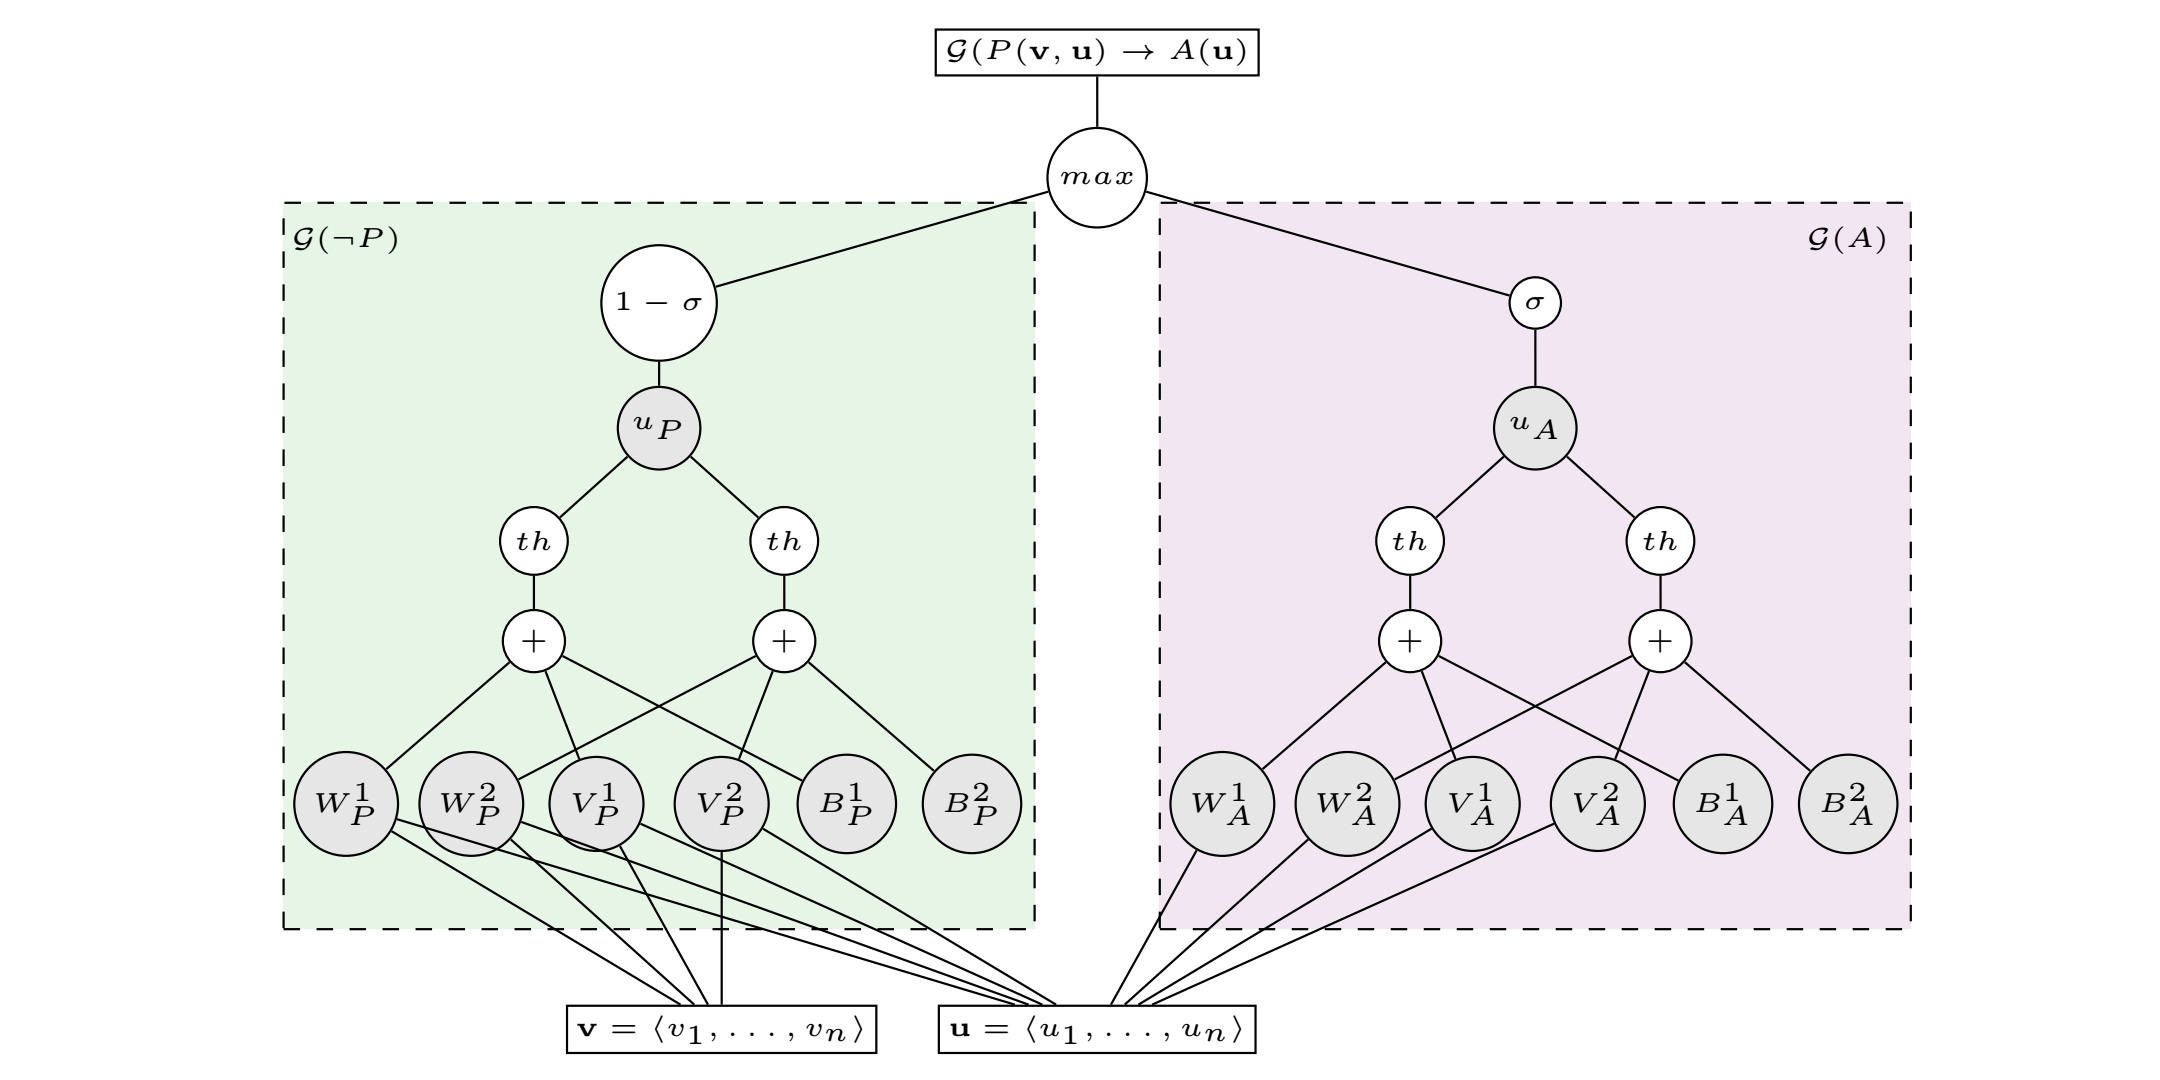
\includegraphics[scale=0.2]{ltn_exp}
	\caption{Retea tensoriala pentru $\neg P(x, y) \rightarrow A(y)$, unde $\mathcal{G}(x) = v$, $\mathcal{G}(y) = u$ si $k = 2$ \cite{LTN}}
\end{figure}

\section{Un exemplu de completare a unei baze de cunostinte}
Retelele logice tensoriale au fost implementate sub forma unei biblioteci in Python numita ``ltn'', utilizand ``TENSORFLOW'', detinut de Google. Pentru a ilustra eficienta ideii, autorii se folosesc de bine-cunoscutul exemplu ``Fumatorii si prietenii''. Fie 14 oameni impartiti in 2 grupuri: $\{ a, b, ..., h\}$ si $\{ i, j, ..., n \}$. In fiecare grup de persoane stim cine fumeaza si cine nu, iar in primul grup stim cine are si cine nu are cancer, pe cand in cel de al 2lea nu dispunem de astfel de cunostinte. De asemenea, exista informatii generale despre fumat, prietenie si cancer, anume ca fumatul cauzeaza cancer, prietenia este o relatie simetrica si antireflexiva (nicio persoana nu este prietena cu ea insasi), toata lumea are cel putin un prieten si ca fumatul se propaga intre prieteni. Toate aceste date sunt reprezentate in baza de cunostinte din Figura 9. Afirmatiile, insa, au diferite grade de adevar, dar acest fapt nu este cunoscut. Altfel, baza de cunostinte rezultata nu ar fi consecventa (de exemplu, ar deduce $S(b)$, dar si $\neg S(b)$). Scopul retelei este urmatorul: sa gaseasca valorile de adevar a afirmatiilor din baza de cunostinte si sa gaseasca valorile de adevar pentru faptele lipsa (de ex, C(i)), dar si sa gaseasca ``grounding''ul fiecarei constante $a, b, ...n$. Pentru a raspunde tuturor acestor cerinte, se foloseste ``ltn'' care aproximeaza baza completa de cunostinte. Pornim de la presupunerea ca toate afirmatiile din baza de cunostinte sunt adevarate (au valoarea de adevar 1). In scopul de a demonstra rolul cunostintelor suplimentare (``de baza'') sunt ilustrate 2 experimente: $\mathcal{K}_{exp1} = \mathcal{K}_{a...h}^{SFC} \cup \mathcal{K}_{i...n}^{SFC}$. In cel de al doilea experiment ($exp2$) introducem si informatiile ``de baza'', deci: $\mathcal{K}_{exp2} = \mathcal{K}_{exp1} \cup \mathcal{K}^{SFC}$.\\
Configuram reteaua astfel: fiecare constanta (persoana) poate avea pana la 30 de atribute reprezentate de valori reale. Numarul $k$ de straturi are retelei neurale tensoriale va fi 10, iar functia $\mu$ folosita va fi $\mu(a, b) = min(1, a + b)$. O aproximare a ``grounding''ului ideal este obtinuta dupa 5000 de rulari are algoritmului de invatare ``RMSProp'' din ``TENSORFLOW''. Rezultatele celor 2 experimente sunt vizibile in tabelele din Figura 10, iar valorile de adevar mai mari ca 0.5 sunt ingrosate pentru lizibilitate. Valorile sunt colorate la fel ca si bazele de cunostinte care provin, iar cele deduse de algoritm au fundal alb. Pentru a evalua calitatea rezultatelor trebuie verificat daca valorile de adevar ale informatiilor preluate din bazele de cunostinte sunt apropiate de 1 si daca valorile de adevar deduse corespund asteptarilor.\\
Se poate observa ca reteaua logica tensoriala asociata lui $\mathcal{K}_{exp1}$ produce aceleasi rezultate ca si $\mathcal{K}_{exp1}$ in sine, deci reteaua produce valorile asteptate. De asemenea, ea deduce informatii suplimentare despre $F$ si $C$ ce nu pot fi derivate din $\mathcal{K}_{exp1}$ din rationamente pur logice, de exemplu: $F(c, b)$, $F(g, b)$, $\neg F(b, a)$. Acestea rezulta din similaritatea groundingurilor constantelor generate de retea. De pilda, $\mathcal{G}(c)$ si $\mathcal{G}(g)$ au o similaritate cosinus ridicata (asemenea functiei ``sim'' din exemplul cu documentele). \\
Rezultatelea celui de al doilea experiment arata ca si mai multe fapte pot fi deduse odata ce includem cunostinte ``de baza''. Mai concret, acum reteaua poate prezice ca  $C(i)$ si $C(n)$ sunt adevarate. In plus, din simetria relatiei de prietenie, reteaua concluzioneaza ca si $m$ este prieten cu $i$ si toate axiomele enuntate din baza de cunostinte suplimentare $\mathcal{K}^{SFC}$ au o valoare de adevar mai mare ca 0.9. Exceptia la aceasta regula este axioma $\forall x (S(x) \rightarrow C(x)$ (fumatul cauzeaza cancer) din moment ce $f$ si $g$ fumeaza si nu au cancer. \cite{LTN}

\begin{figure}
	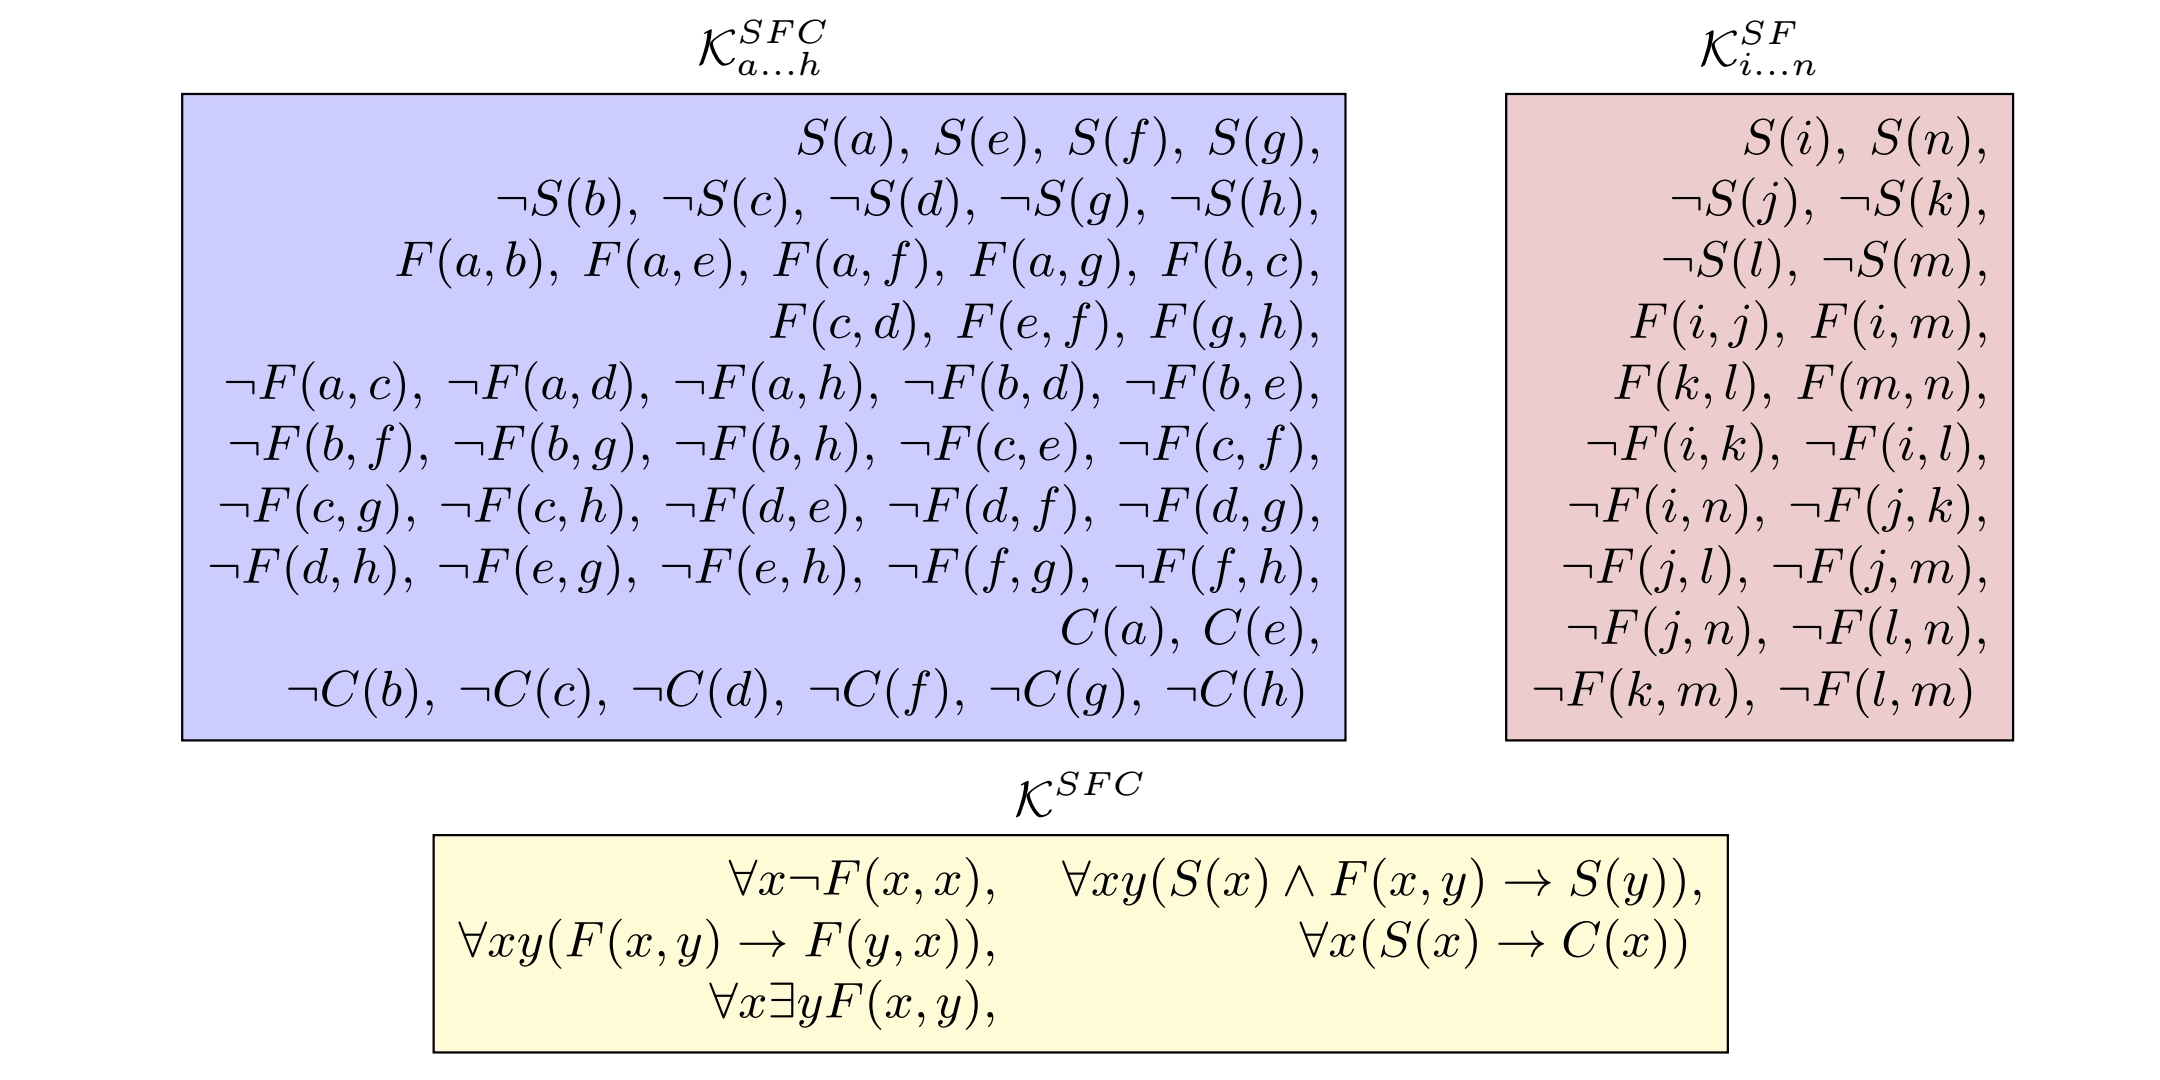
\includegraphics[scale=0.2]{kb}
	\caption{Baza de cunostinte initiala \cite{LTN}}
\end{figure}

\begin{figure}[H]
	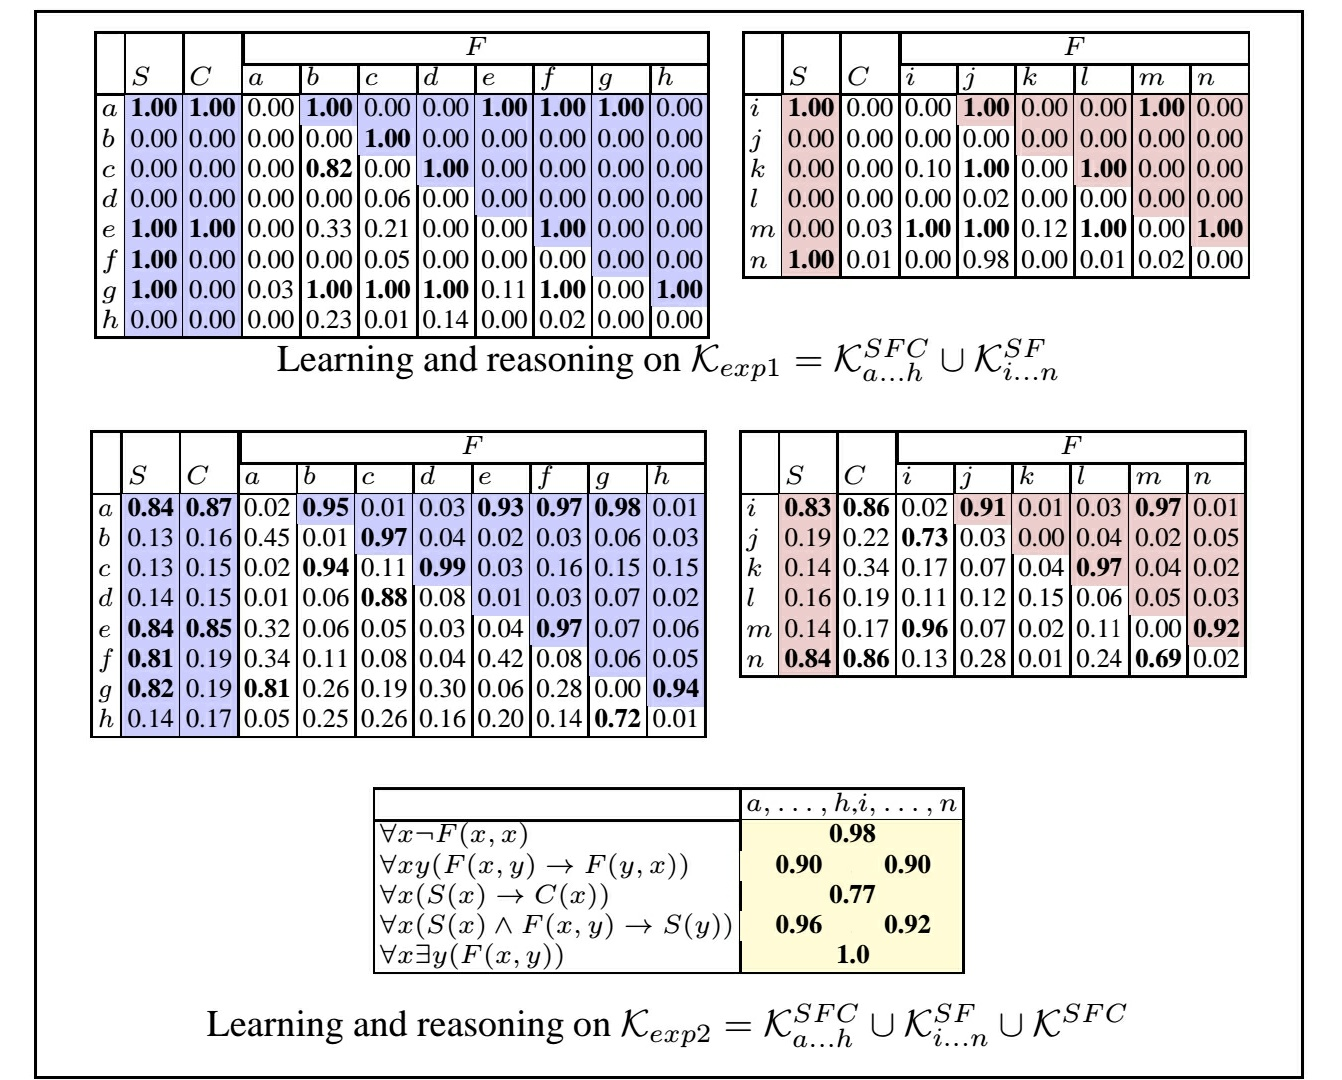
\includegraphics[scale=0.2]{table}
	\caption{Baza de cunostinte completata de reteaua logica tensoriala \cite{LTN}}
\end{figure}

%Questions I thought of while writing
%Original examples
%Better presentation of first order logic
%What I intend to do in each subsection and section + conclusions at the end 
%Uses I see for the proposed model

\begin{thebibliography}{9}
\bibitem{LTN}
	Luciano Serafini si Artur d'Avila Garcez - Logic Tensor Networks: Deep Learning and Logical Reasoning from Data and Knowledge
	
\bibitem{NTN}
	Richard Socher, Danqi Chen, Christopher D. Manning, Andrew Y. Ng - Reasoning with Neural Tensor Networks for Knowledge Base Completion

\bibitem{Tensor}
	http://mathworld.wolfram.com/Tensor.html

\bibitem{Tensor_Rank}
	http://mathworld.wolfram.com/TensorRank.html
	
\bibitem{Tensor_Multiplication}
	Joseph C. Kolecki - An Introduction to Tensors for Students of Physics and Engineering

\bibitem{Deep_Learning}
	https://www.analyticsvidhya.com/blog/2016/03/introduction-deep-learning-fundamentals-neural-networks/
	
\bibitem{FOL}
	David W. Kueker - Cursul Mathematical Logic I (http://www-users.math.umd.edu/~dkueker/)
	
\bibitem{Clause}
	https://en.wikipedia.org/wiki/Clause\_(logic)
	
\bibitem{Closed_Term}
	http://john.fremlin.de/schoolwork/logic/logic/node7.html
	
\bibitem{Free_Variable}
	https://en.wikipedia.org/wiki/First-order\_logic\#Free\_and\_bound\_variables

\end{thebibliography}

\end{document}